\documentclass[doku.tex]{subfiles}
\begin{document}
	\subsection{日常}
\begin{description}
		\item[照片] \label{passforo}在延签的时候需要免冠照片,单张的大小差不多35mm*53mm也就是国内所说的2寸照片,请注意底必须是白色的,必须。 dm也可以拍,就是Passfoto,但是拍的实在是过于写实~
		\item[信用卡,现金] 刚来德国带一个中国信用卡还是很有必要的,现金尽量不要拿500欧的那种,20欧,100欧这样用起来更方便些,很多店家不收这种,,,也许长这么大都还没见过。
		\item[药物] 我带了感冒药(病毒性和细菌性),腹泻,和抗过敏,目前这个情况下,还需要自己带一些ffp2防护等级的口罩。
		\item[眼镜] 这个还是需要备一副,重新配贵不说,就怕和配眼镜的人说不清楚。。。(镀膜,树脂,防蓝光,抗污,偏色,鼻垫。。。这些词的德语怎么说。。   
		\item[针线] 有备无患,我虽然带了,但也只是用过里面的针来取手机卡。
		\item[菜刀] 我觉得既然来了就要做饭,带个中式菜刀还是蛮有必要的,磨刀问题的话,感兴趣可以在淘宝买个360/800的双面磨刀石,记得备注一下不要容易下料的,或者自己弄觉得麻烦,可以等来了德国买个那种磨刀器\href{https://www.amazon.de/Limirror-Messersch%C3%A4rfer-Messerschleifer-Messerschaerfer-Vintage-Schwarz/dp/B08JQ5L7NY/ref=sr_1_7?__mk_de_DE=%C3%85M%C3%85%C5%BD%C3%95%C3%91&crid=2IX7ZZKQLY1KK&dchild=1&keywords=messer+versch%C3%A4rfer&qid=1612527983&sprefix=messer+vers%2Caps%2C186&sr=8-7}{Messerschärfer}
		厨房剪刀有地方就带,没有就算了。
		\item[筷子] 也不沉,多带几双,木头筷子可以在淘宝搜一搜鸡翅木的筷子,很便宜,我的这些筷子用了4年了,没有长毛,也没有发霉,当然金属和塑料的更稳,但是我更喜欢用木头的~ \label{chopstick}
		\item[笔] 如果只喜欢用中性笔需要自己带,这边基本卖的都是圆珠笔,还是贼滑的那种
		\item[零钱包] 最好能买一个既可以放卡片和纸现金,又有专门放硬币地方的那种
		\item[水瓶] 如果有喝热水保温需求的可以自己带一个,保温的那种,普通的塑料水瓶我觉得意义不大,一般我都直接买1.5l的水喝
		\item[水杯] 那种陶瓷的杯子,行李有空就带一个,没有也无所谓,只要不在乎外观,在德国很容易买到
		\item[耳勺,牙签] 习惯用耳勺的可以自己带几个,这边dm卖的牙线都是带牙签的那种,而且也不贵,习惯牙线之后,还是很爽的
		\item[被] 需要从国内带一个保温比较好的,刚来三四月还是挺冷的,夏天晚上也挺冷,夏天温差有10摄氏度左右,夏天需要一个小薄被,不是单子,而是小薄被,但是这种的小薄被可以在ikea买
		\item[枕头] 我来的时候因为重量原因,只带了一个那种超软易于压缩的那种,后来很快我就又买了一个那种类似人体工学的在德国,价格是20欧,带的话我觉得只是一个能用凑付一两晚的那种,不占行李重量的那种就行
		\item[豆浆机] 我觉得第一次来不需要带,还是带一些更重要的东西吧,黄豆的德语是Soja,在dm能买到豆浆,REWE能买到黄豆,Penny有豆腐叫做Toufu
		
\end{description}

	\subsection{洗漱}
\begin{description}
		\item[毛巾] 大的小的都带一些,反正不贵又不怎么占空间和重量
		\item[沐浴露,香皂] 就带个旅行装够一两次的就行,来了之后我们肯定会带着你们去dm采购的
\end{description}

	\subsection{吃喝}
我觉得就带一些常用的干燥的香料就好,感觉家里常用的用的比较顺手,液体类的就不用带了,在科布买起来还是很方便的\href{http://www.thanh-hoa.de/}{Thanh-Hoa Asia-Markt}, 我觉得最后如果行李还有余量可以用牛油火锅底料和蘸料来填充,团结同学必备良品,牛羊肉可以去这里的土超\textbf{Sham Paradies für Lebensmittel und frisches Fleisch}购买。 剩下的就带一点路上能补充能量不让自己饿着的零食就好,能量棒啦,巧克力啦啥的。 红糖啥的亚超还是都能买到的。

至于电饭煲和电磁炉,我对米饭馒头这类的面食,没有过多的念想,我刚来的的时候没有带这些东西,电磁炉是第二次来德国的时候带的,为的是和同学吃火锅,和替补住的这里不给力的电陶炉。。 电饭煲我一直没有拿。 如果担心自己的做饭能力可以带一个最小的那种电饭锅。至于锅碗瓢盆,来的时候第一天我们会带着你们去采购。

有小伙伴问我们\textbf{电饭锅\label{Reis}}的问题,有空余位置的话可以自己带,如果想自己煮,我的建议是买超市里Jasmine的米,和咱们在国内日常吃的那种米的口感很像,其他的例如Milchreis,是长粒的米,一粒一粒的过于分明,我多水和少水都试过,但是Milchreis的口感确实不好,我平常米是直接煮,我一般,水的高度是米的高度的一倍,炉子开中火,初期要稍微搅一搅防止糊底,等开锅之后就不用搅了,然后还是中火,等15min左右就差不多了~
	\subsection{衣物}
首先说明,我对衣服穿搭。。没啥要求。。。 不需要带十分厚的那种内衣,我带过来的超厚的内衣,从来没有穿过。
\begin{figure}
	\centering
	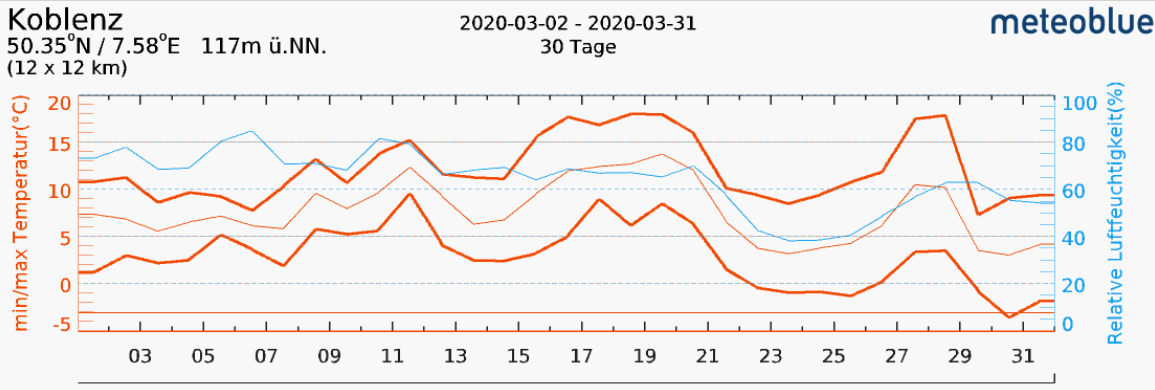
\includegraphics[width=0.7\linewidth]{screenshot001}
	\caption{科布伦茨2020三月气温}
	\label{fig:screenshot001}
\end{figure}
\begin{figure}
	\centering
	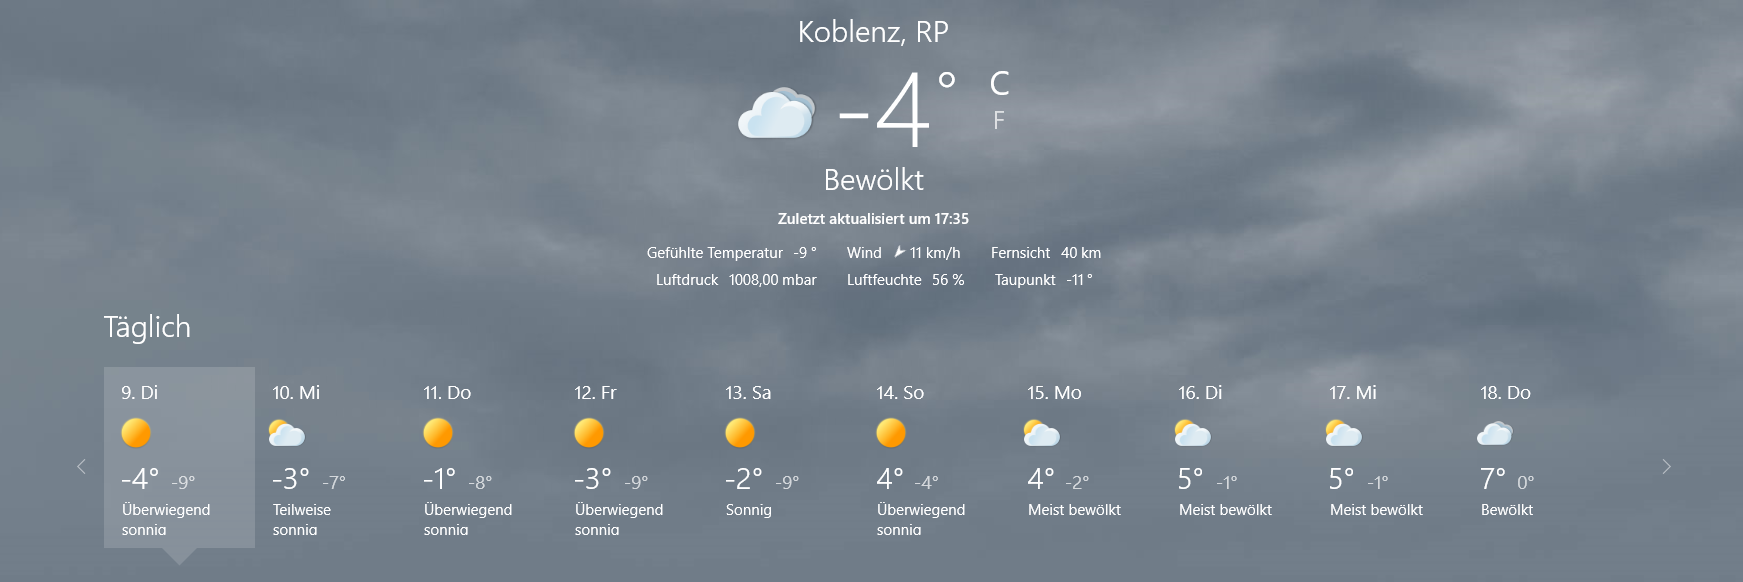
\includegraphics[width=0.7\linewidth]{screenshot002}
	\caption{德国最冷也就不过如此了}
	\label{fig:screenshot002}
\end{figure}
我目前的穿搭就是短袖打底,一件抓绒,一个羽绒的冲锋衣。裤子就是带一点绒的户外裤子。\\
夏天我就是五条短裤,五间短袖轮换着穿,夏天这里阳光还是十分强的那种,看自己需要可以带个皮肤衣什么的。\\
冬天我就是夏天的短袖打底,四件迪卡侬抓绒,和一个羽绒冲锋衣,其实多数地方德国暖气给的还是很足的。\\
其他时候我基本上就是几条牛仔裤,随便配上衣,
牛仔裤在这里卖的还是蛮多的,只是对于我而言他们的裤子都有些长。\\
鞋 这边鞋其实还是挺贵的,我目前就是国内带的两双,一双在这边买的阿迪跑步,一双迪卡侬徒步,拖鞋不沉不占地,带两双夏季的那种就好,不用带冬季用的那种厚的。。\\
内衣内和袜子就看自己需求,尽量多带吧。

\subsection{杂七杂八}
这边单纯理发17欧,不包含清理,我们在这边一直是互相理发,男生还是很有必要自己带电动理发推子和一套剪子,几个男生至少有一套吧。

\begin{figure}[H]
	\centering
	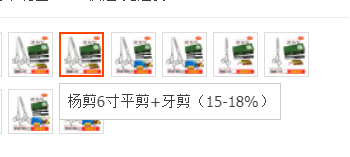
\includegraphics[width=0.7\linewidth]{screenshot003}
	\caption{正品杨剪美发剪刀平剪牙剪专业理发剪刀套装进口钢材打薄剪包邮,\href{https://item.taobao.com/item.htm?spm=a1z09.2.0.0.70932e8d1wonf8&id=12950418954&_u=avoelvl5e94}{URL}}
	\label{fig:screenshot003}
\end{figure}

来德国要注意假期时间,因为假期里,超市是不上班的, 需要提前做好准备。\\

安全性,我觉得科布的安全上没太大问题,但是也不能完全放松,出门还是要保护好自己的,注意和朋友以及舍友报告自己的行踪,不要隐匿自己的行踪,科布这里没有什么,让我看一眼就会感觉到害怕的人和地方,,柏林法兰这样的大城市人会杂会乱一些,德国这里经济越是发达的地方,人会越杂,像是旅游城市(像是科布)或者小城镇问题不会很大,但也不可掉以轻心哦。

\end{document}